\documentclass{article}

\usepackage[margin=1in]{geometry}
\usepackage{graphicx}

\begin{document}

\begin{figure}
    
\caption{Weak vs Strict Inequality, with Rounded Conforming Loan Limits -- by Window}

\bigskip

\emph{Type 1 Error: Share of Jumbo Loans in McDash that are below the limit, either with strict inequality (bold line) or with a weak inequality (dotted line).}

\emph{Type 2 Error: Share of loans below the limit, either with strict inequality (bold line) or with a weak inequality (dotted line), that are Jumbo Loans in McDash.}

\begin{center}
    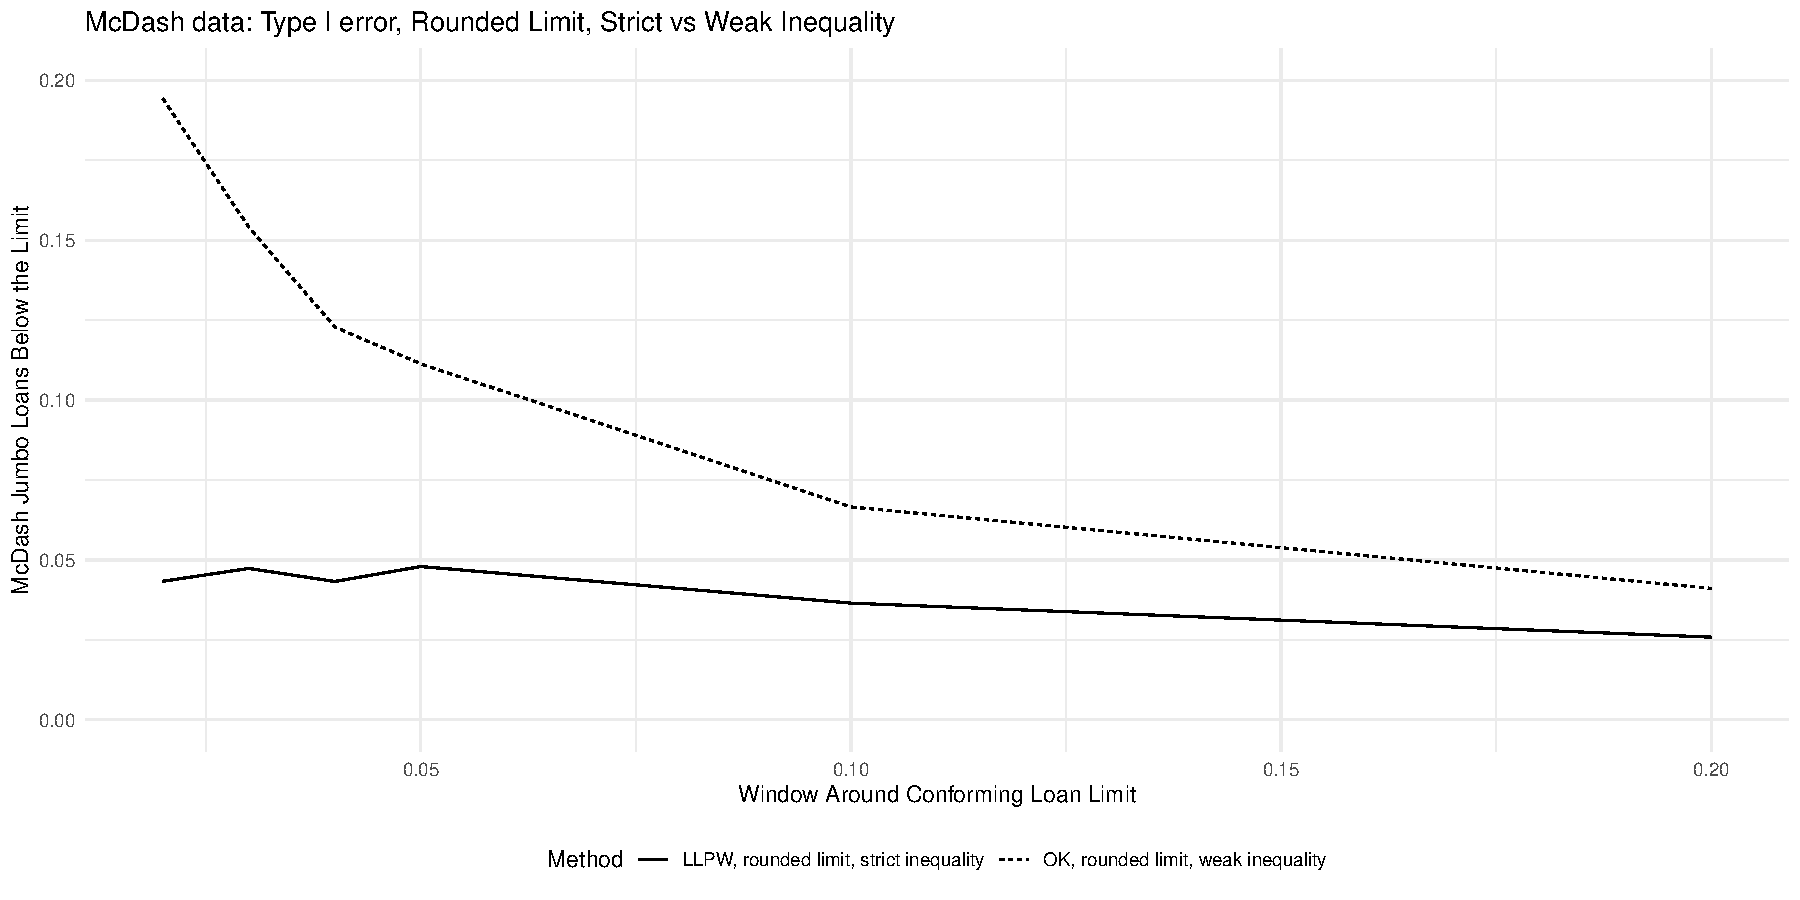
\includegraphics[scale=0.5]{figures/type1error_bywindow_weak_vs_strict.pdf}
\end{center}

\bigskip

\begin{center}
    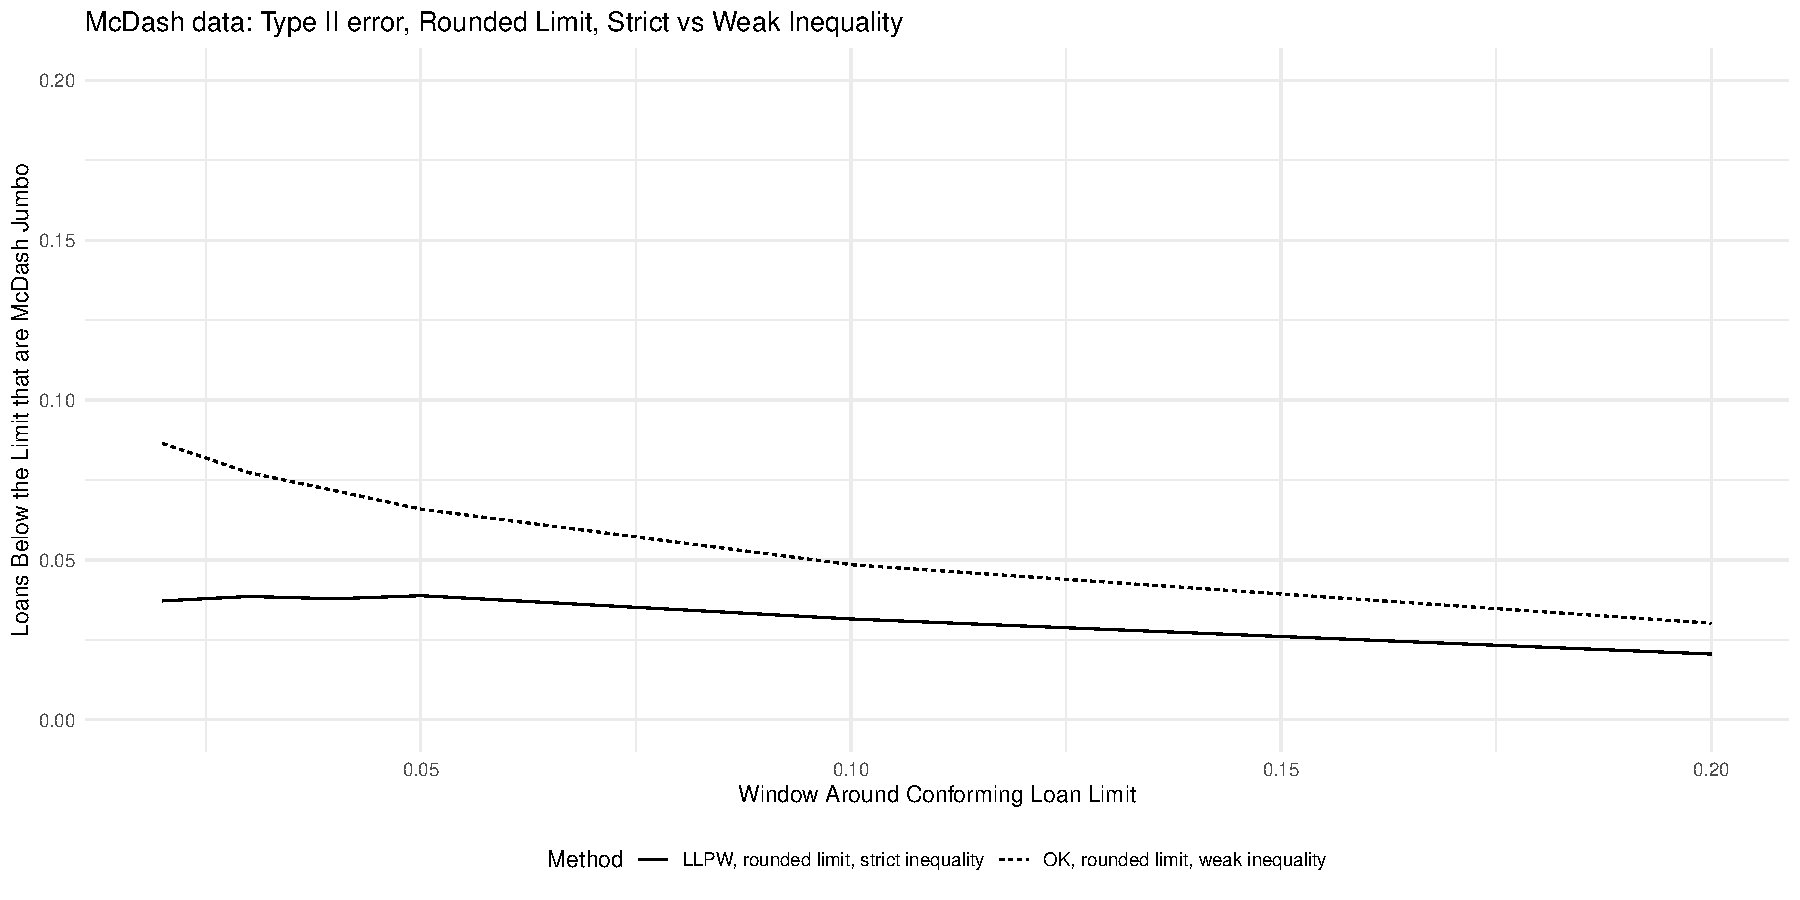
\includegraphics[scale=0.5]{figures/type2error_bywindow_weak_vs_strict.pdf}
\end{center}

\end{figure}

\clearpage
\pagebreak

\begin{figure}
    
    \caption{Weak vs Strict Inequality, with Rounded Conforming Loan Limits -- by Year}

    \bigskip
    
    \emph{Type 1 Error: Share of Jumbo Loans in McDash that are below the limit, either with strict inequality (bold line) or with a weak inequality (dotted line).}

\emph{Type 2 Error: Share of loans below the limit, either with strict inequality (bold line) or with a weak inequality (dotted line), that are Jumbo Loans in McDash.}

    \begin{center}
        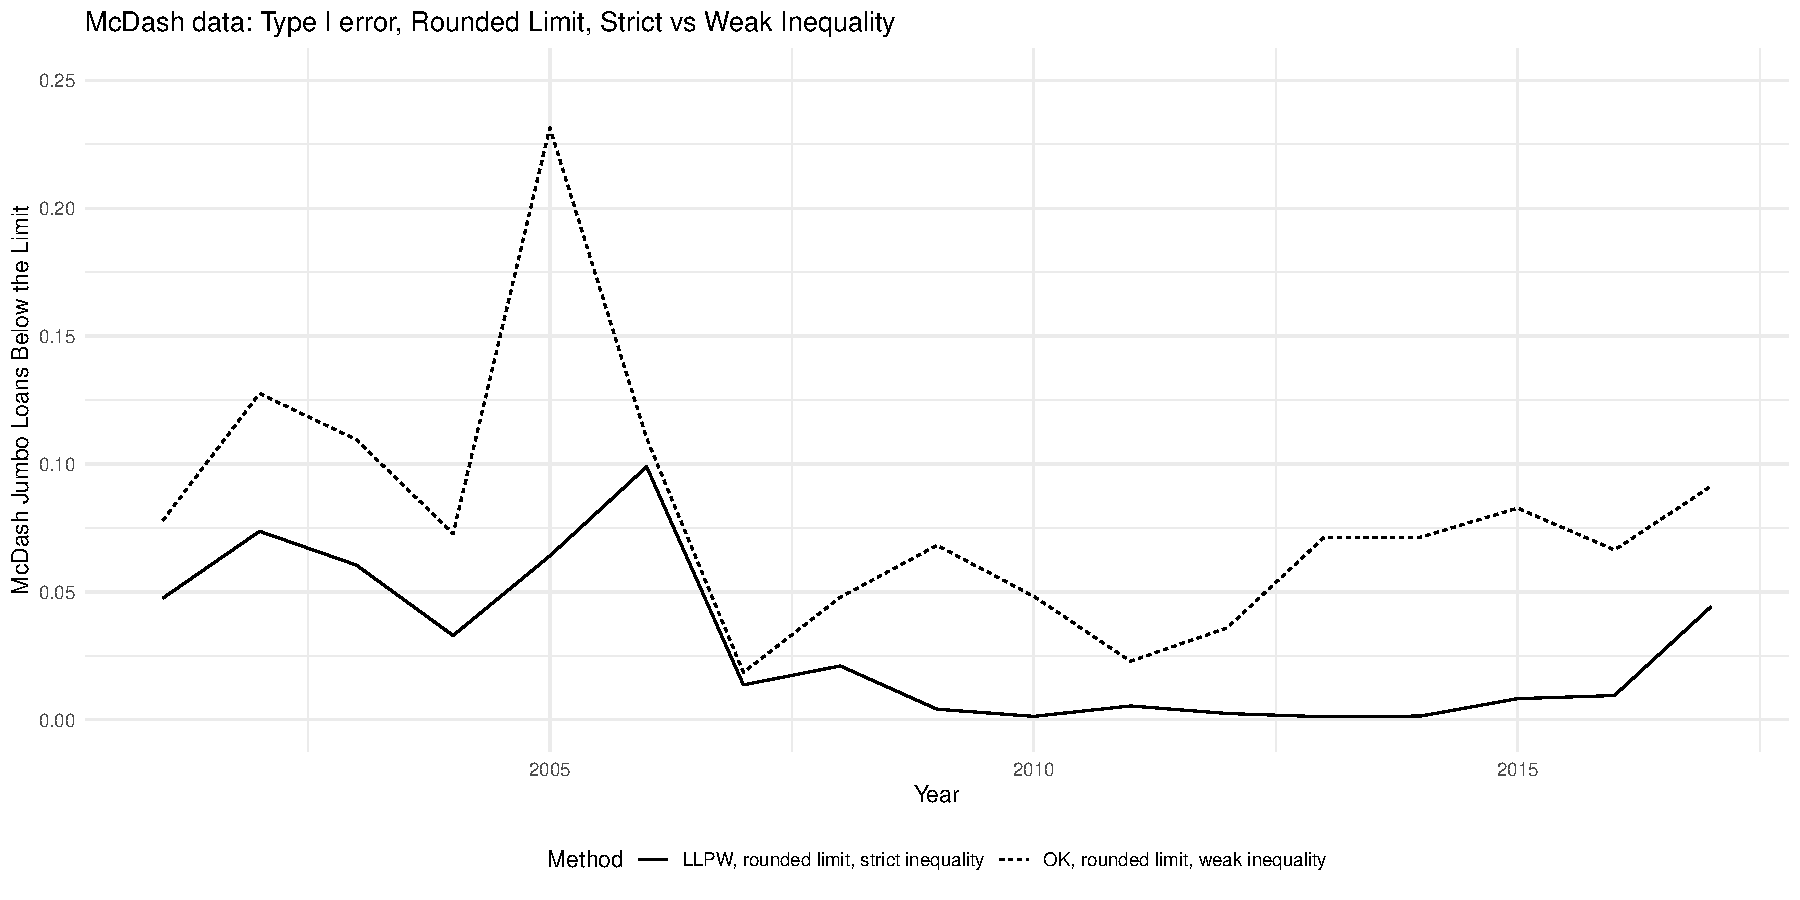
\includegraphics[scale=0.5]{figures/type1error_weak_vs_strict.pdf}
    \end{center}
    
    \bigskip
    
    \begin{center}
        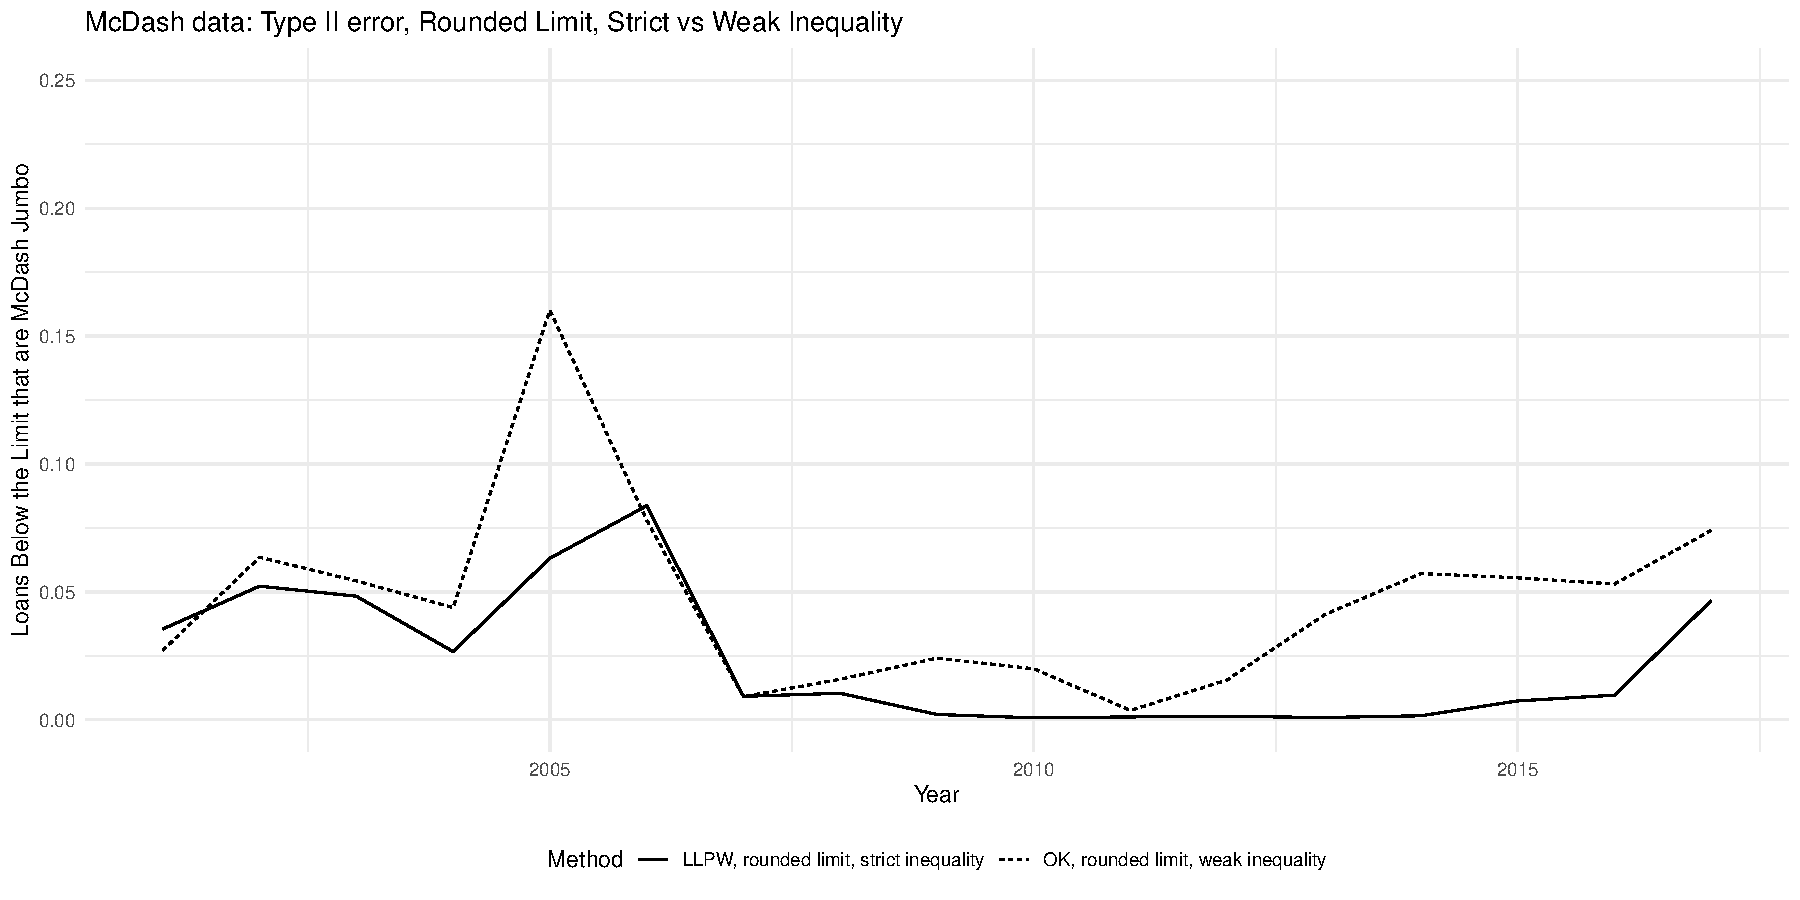
\includegraphics[scale=0.5]{figures/type2error_weak_vs_strict.pdf}
    \end{center}
            
    
\end{figure}
    

\end{document}